\section{eo\-Quad\-Gen\-Op$<$ EOT $>$ Class Template Reference}
\label{classeo_quad_gen_op}\index{eoQuadGenOp@{eoQuadGenOp}}
Wrapper for quadop: easy as pie.  


{\tt \#include $<$eo\-Gen\-Op.h$>$}

Inheritance diagram for eo\-Quad\-Gen\-Op$<$ EOT $>$::\begin{figure}[H]
\begin{center}
\leavevmode
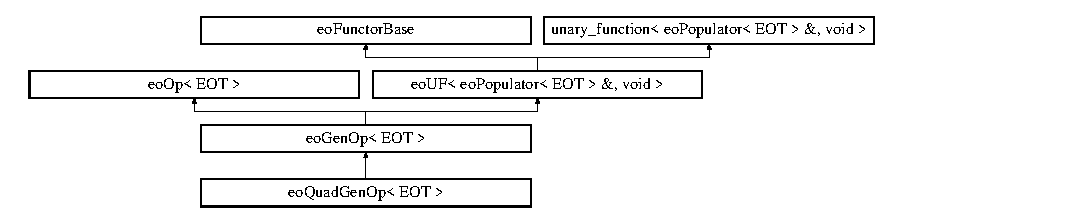
\includegraphics[height=2.54835cm]{classeo_quad_gen_op}
\end{center}
\end{figure}
\subsection*{Public Member Functions}
\begin{CompactItemize}
\item 
{\bf eo\-Quad\-Gen\-Op} ({\bf eo\-Quad\-Op}$<$ {\bf EOT} $>$ \&\_\-op)\label{classeo_quad_gen_op_a0}

\item 
unsigned {\bf max\_\-production} (void)\label{classeo_quad_gen_op_a1}

\begin{CompactList}\small\item\em Max production is used to reserve space for all elements that are used by the operator, not setting it properly can result in a crash. \item\end{CompactList}\item 
void {\bf apply} ({\bf eo\-Populator}$<$ {\bf EOT} $>$ \&\_\-pop)\label{classeo_quad_gen_op_a2}

\begin{CompactList}\small\item\em the function that will do the work \item\end{CompactList}\item 
virtual std::string {\bf class\-Name} () const \label{classeo_quad_gen_op_a3}

\end{CompactItemize}
\subsection*{Private Attributes}
\begin{CompactItemize}
\item 
{\bf eo\-Quad\-Op}$<$ {\bf EOT} $>$ \& {\bf op}\label{classeo_quad_gen_op_r0}

\end{CompactItemize}


\subsection{Detailed Description}
\subsubsection*{template$<$class EOT$>$ class eo\-Quad\-Gen\-Op$<$ EOT $>$}

Wrapper for quadop: easy as pie. 



Definition at line 157 of file eo\-Gen\-Op.h.

The documentation for this class was generated from the following file:\begin{CompactItemize}
\item 
eo\-Gen\-Op.h\end{CompactItemize}
